Skemalægningen har længe været et problem, som diverse skoler har haft svært ved at løse, heriblandt er Sofiendalskolen, som vi har interviewet.
Selvom der findes mange gode skemalægningsprogrammer er det ikke nødvendigvis ensbetydende med at alle skoler kan benytte disse programmer af den grund, at nogle skoler har svært ved at begrænse sig til så få parametre, som programmerne indeholder. Herudover nævner interviewpersonen, Søren Kusk, at: ”[…] selvom det tager højde for mange ting, så er der bare nogle ting som det ikke altid tager højde for.” Dette tydeliggør problematikken og pointen i, at skemalægningsprogrammerne ganske enkelt ikke indeholder nok parametre og er præcis nok, til at skoler med forhindringer kan gøre brug af programmerne. 

  \subsubsection{Docendo}
    \subsubsection{Docendo}
Skemalægningsprogrammet Docendo er et brugervenligt samt forholdsvis simpelt program. Programmet går ud på, at der dannes en kalender med uger og dage, hvorefter brugeren har mulighed for at justere diverse parametre alt efter behov. Heriblandt tager programmet bl.a. højde for, at nogle skoler har forskellige fag, og giver derfor brugeren mulighed for at tilføje et eller flere fag. Samtidig har brugeren mulighed for at tilpasse lektionernes længde, hvilket også er en essentiel parameter, da nogle skoler forsøger på at undgå tunge fag om eftermiddagen eksempelvis. Dernæst fastlåser programmet lokaler og lærere som har undervisning på bestemte tidspunkter, så brugeren fortsat har overblik over skemaplanlægningen og så der ikke opstår dobbeltbookninger af et bestemt lokale eller lignende. Hvis et problem skulle opstå, kan lektionerne flyttes med et simpelt klik, og de nye skemaer bliver genereret i ét, hvilket igen gør at der er fortsat overblik over skemalægningen.


  \subsubsection{Lantiv}
    Lantiv Timetabling Turbo 7 er et planlægningsprogram der med hensyn til nogle begrænsninger angivet af brugeren, kan udvikle et skema til blandt andet folkeskoler. For hver begrænsning, kan brugeren angive en minimum, maksimum og ønsket værdi. En variation fra den ønskede værdi, bliver af programmet registreret som en mindre overtrædelse, mens en værdi der ligger under minimumsværdien eller over maksimumsværdien, bliver registreret som en alvorlig overtrædelse. Programmet starter med at afsætte kort tid til løsning af overtrædelser, hvorefter den afsatte tid stiger for at løse de sværere overtrædelser. Denne proces stopper, når programmet enten har løst alle overtrædelser, eller den maksimale afsatte tid er nået. Hvis overtrædelser af brugerens begrænsninger ikke kan undgås, bliver der lavet et kompromis, hvor programmet hovedsageligt forsøger, at overholde de begrænsninger, brugeren har angivet med høj prioritet, mens overtrædelser af begrænsninger med lav prioritet bliver accepteret. Begrænsningerne kan tilpasses af brugeren, efter skemaet er genereret, og programmet vil levere nogle tilpassede løsninger som forslag. Det oprindelige skema vil kun blive slettet, hvis en af disse løsninger, accepteres af brugeren. Under processen kan brugeren bestemme, hvor meget de tilpassede skemaer må variere fra det oprindelige. Der kan f.eks. stilles et krav, om at programmet kun ændrer lektionerne for en enkelt lærer. I dette tilfælde, vil ingen af de tilpassede forslag, have ændret i andre dele af skemaet. Når skemaet er genereret, er det også muligt for brugeren selv, at tage fat i en lektion og flytte den. Her vil programmet vise, hvor lektionen kan placeres uden at forårsage dobbeltbookninger af lokaler, lærere eller klasser. Hvis brugeren placerer en lektion der forårsager en konflikt, bliver problemet forklaret i detaljer af programmet, og hvis det er en dobbeltbookning, er der muligheden for at slette en af lektionerne eller accepterer dobbeltbookningen\cite{lantiv2016}.
\begin{figure}[h]
  \centering
  \includegraphics[scale = 0.9]{partials/graphics/lantiv.png}
  \caption{Skemalægning i programmet Lantiv\cite{lantiv2016}.}
  \label{fig:lantiv}
\end{figure}



  \subsubsection{Tabulex}
    Skemalægningsprogrammerne er dog ikke problemfri. Selvom programmet opfylder de mest væsentlige krav omkring, hvorvidt et skema bør lægges for at få optimalt udbytte, er programmet for upræcist i forhold til hvilke parametre der tages stilling til, og hvilken af parametre prioriteres højest. Typisk vil sådan et program virke for en skole, hvor lærere ikke har problemer med hensyn til opdeling i teams mm., men dette er ikke tilfældet nogle steder. Heriblandt er Sofiendalskolen, som er af skolerne, hvor lærernes teams ikke fungerer optimalt på grund af, nogle af lærerne er medlemmer i flere teams. Dette er en essentiel parameter som der ikke tages højde for i skemalægningsprogrammerne, som forårsager forringet udbytte af programmet og i værste fald en helt anden alternativ metode at lægge skemaet. Dog er der samtidig andre faktorer, som gør det en hel del svære at benytte skemalægningsprogrammerne, da programmerne ellers skal være skræddersyet for en specifik skole, før det kan lade sig gøre.
Derfor vil en mulig forbedring af de nuværende skemalægningsprogrammer være at tage stilling til mindre faktorer. Programmet skal derfor ikke kunne udlevere et endeligt skema, men til gengæld skal det kunne give en klar formular eller en retningslinje, som skolen herefter kan følge og tilpasse, alt afhængigt af hvilke parametre og faktorer skolen prioriterer højest\cite{tabulex}. 


  \subsubsection{Untis}
    Untis er et fleksibelt skemalægningsprogram, som både er nemt at bruge, og giver mange muligheder for brugeren. Untis giver bl.a. mulighed for at brugeren kan bestemme, hvordan skemaet skal se ud uge for uge. Brugeren kan vælge om ugerne skal være A- og B-uger, altså eksempelvis, hvis der gennemsnitligt skal være 5 matematiklektioner på en uge, kan brugeren via A- og B-uger-funktionen gør således at der kommer 4 matematiklektioner i en uge, og 6 i en anden. Desuden har brugeren mulighed for at ændre skemaet, hvis nødvendigt i udvalgte uger, og bibeholde de resterende uger som faste og ensartede. 
Untis giver brugeren flere muligheder for at lægge skema, heriblandt manuel skemalægning, automatisk skemalægning samt optimering og en blanding af de nævnte. Dette sker ved at brugeren udfylder udvalgte brikker, og herefter benytter Untis til at udfylde resten for at opnå det bedste mulige resultat. Efter de manuelle indtastninger er udført, tager programmet stilling til de angivne parametre og forsøger at levere det bedste skema. Hvis der opstår konflikter, vil Untis informere brugeren og og vise hvori problemet ligger, så brugeren har nemt ved at rette fejlene og justere parametrene. Desuden tager programmet hensyn til indtastede data før programmet begynder at generere mulige skemaer, for at sikre at brugeren har indtastet korrekte eller realistiske antal af eksempelvis lokaler, lærer, klasser mm.\footfullcite{untis2016}
\begin{figure}[!h]
  \centering
  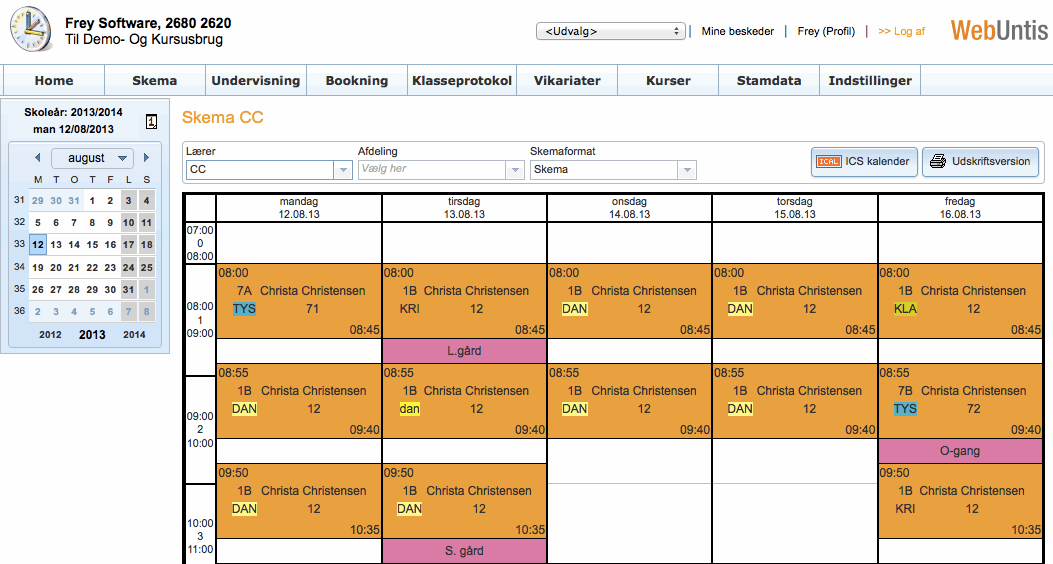
\includegraphics[width=\textwidth]{partials/graphics/untis.png}
  \caption{Eksempel på skemplanlægning i Untis.\footfullcite{untisb}}
  \label{fig:untis}
\end{figure}
